\documentclass[12pt]{report}

\usepackage[utf8]{inputenc}
\usepackage{graphicx}
\graphicspath{ {images/} }


\makeatletter
\renewcommand{\@makechapterhead}[1]{
  {\noindent\raggedright\normalfont
   \Large\bfseries \@chapapp\space\thechapter
   \par\nobreak
   \vskip 5\p@
   \Large \bfseries #1\par\nobreak}
  \vspace{\baselineskip}
}
\makeatother

\begin{document}
    \begin{titlepage}
    \begin{center}
 
        \textbf{IMPLEMENTING A COHESIVE PROGRAMMING ECOSYSTEM IN MECHANICAL ENGINEERING}
 
        \vspace{1cm}
         by
             
        \vspace{1cm}
        \textbf{ZAKARY CHRISTIAN OSTER}
 
        \vspace{1cm}
        B.S., Kansas State University, 2022
             
        \vspace{1cm}
        A THESIS
             
        \vspace{1cm}
        submitted in partial fulfillment of the requirements for the degree
 
        \vspace{1cm}
        MASTER OF SCIENCE
 
        \vspace{1cm}
        Department of Mechanical Engineering\\
        College of Engineering
      
        \vspace{1.5cm}
             
        KANSAS STATE UNIVERSITY\\
        Manhattan, Kansas\\
        2024
    \end{center}
 
    \begin{flushright}
        Approved by:
 
        \vspace{1.5cm}
        Major Professor\\
        Jeremy A. Roberts
    \end{flushright}
 \end{titlepage}

    \begin{flushleft}
    \Large
    \textbf{Abstract}
    \normalsize
    \thispagestyle{empty}
\end{flushleft}

The ability to apply modern solution methods is critical for the success
of mechanical engineers. While handwritten solutions were once the 
state of the art, computer programs provide unparalleled power and speed 
to solve problems. Because of this, it is critical that academic 
curriculum teaches students to use programming to solve problems.
The current implementation of programming in the department varies,
with three different languages being used. The usage rate also varies,
with many classes failing to take advantage of the tools provided by
programming, and this is reflected by the ability and confidence of
students in the department.
This project demonstrates how it is possible to use one programming 
language and environment through the mechanical engineering
undergraduate curriculum. The completed projects and assignments
showcase the varying uses of Python, the Raspberry Pi Pico, Visual
Studio Code, and Jupyter Notebooks as it relates to problem-solving
in the field of mechanical engineering.

    
    \input{bookends/acknowledgements}

    \tableofcontents

    \listoffigures

    \listoftables
    
    \chapter{Introduction and Background}
    \section{Introduction}

Engineers solve problems. Regardless of field, discipline, and generation, every engineer
strives to solve problems. While the need for problem solvers does not change with time,
the methods for solving problems certainly do. Consider the process of creating detail 
drawings. Engineers needed a way to communicate the size, shape, and finish of parts to 
other engineers, so they hand drew and dimensioned parts. But in the modern day, the 
thought of hand drafting a detail drawing is laughable. And education has adjusted in
kind. While students are taught to draw straight lines (which all lines are) and visualize
without the aid of CAD, no class spends time teaching students how to use a drafting table
or create detail drawings by hand. Rather, they are taught the basics of visualization
and then taught how to use SOLIDWORKS.

The same could be said for setting the state in a thermodynamics problem, graphing
deflection in a load-bearing beam, or finding the Q-value of a fission reaction. At one
point, looking up values in a table and plugging them into a calculator or using a ruler
and lined paper were state-of-the-art methods for solving these problems. However, as the 
times change, so do the methods, and with the advent of programming and its ever lowering 
barrier to entry, these problems can more easily, and more accurately, be solved with a 
simple script in any number of programming languages.

Despite this, most classes continue to have students spend hours thumbing through tables
and solve every problem by hand. In contrast to this, other classes have recognized the
value of modern solution methods and rely heavily on them, only to find that students
lack sufficient training to effectively utilize them. Because of this dichotomy, a cohesive 
and consistent programming ecosystem should be implemented throughout the curriculum 
of the Mechanical and Nuclear Engineering department.


\section{Background}

The first introduction to programming in MNE curriculum is DEN 161: Engineering Problem Solving,
the first-semester introduction-to-engineering class. The class spends a few weeks introducing
Python and then a week introducing the Arduino Uno. After this, no programming is used in the
curriculum until first semester Junior year, as seen in figure \ref{fig:mne_flowchart}. 

\begin{figure}[h]
    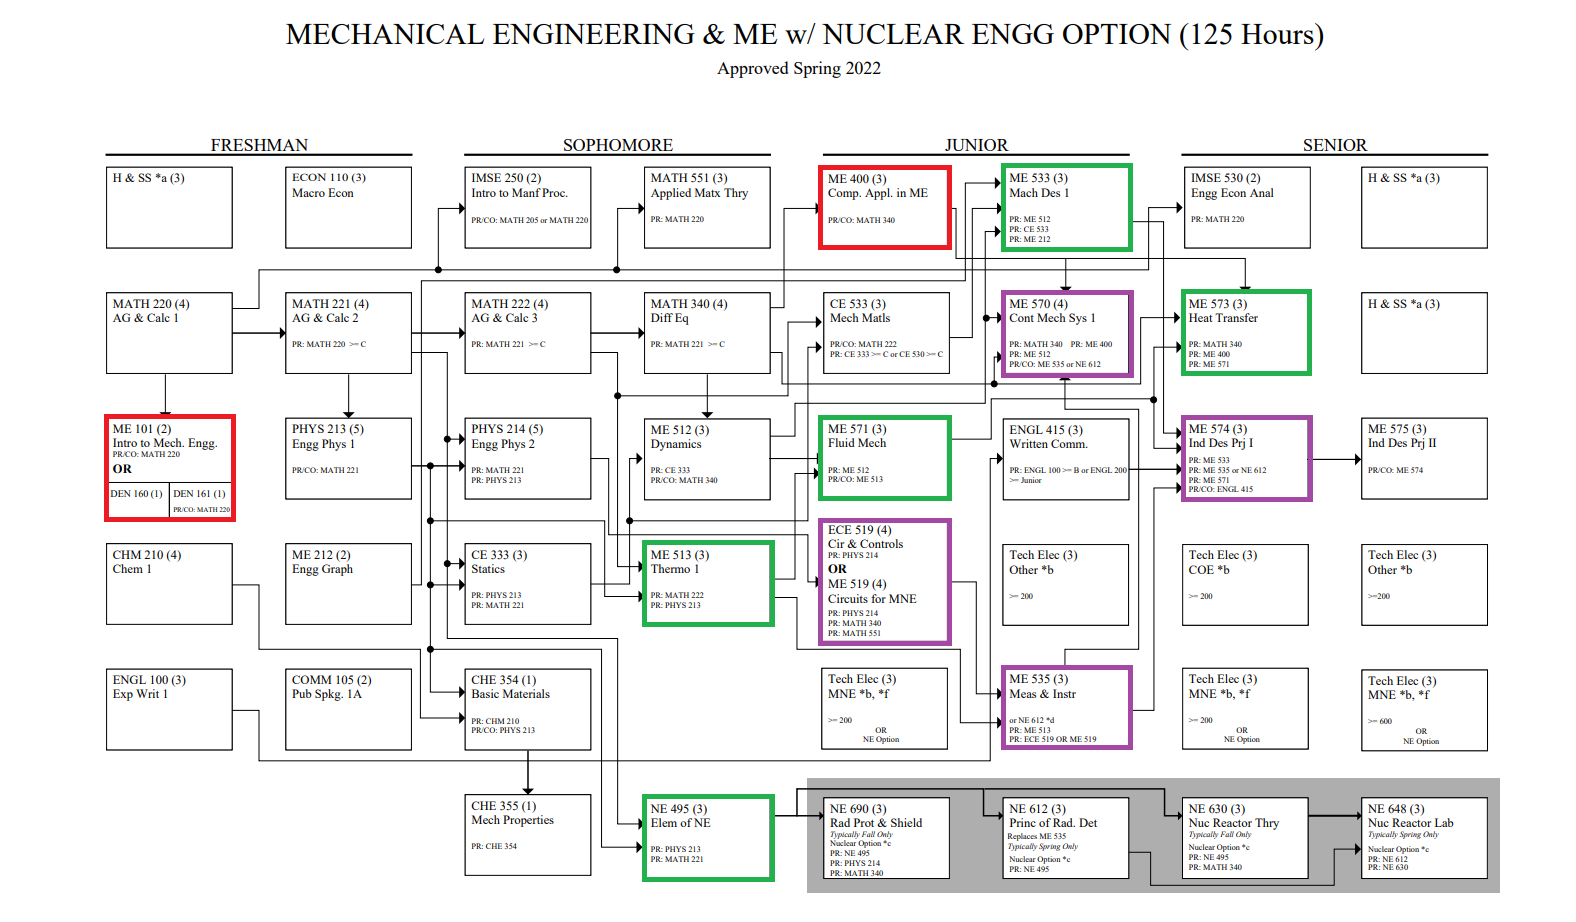
\includegraphics[width=\textwidth]{mne_flowchart}
    \begin{tabular}{l@{ : }l}
        Red & Teaches Programming \\
        Purple & Uses Programming \\
        Green & Does not utilize Programming, but could \\
    \end{tabular}
    \centering
    \caption{MNE Curriculum Flowchart}
    \centering
    \label{fig:mne_flowchart}
\end{figure}

The next class to use programming is also the only class dedicated to teaching programmig.
ME 400: Computer Applications in Mechanical Engineering begins with an introduction to C++
but then quickly moves to teaching embedded C++ for use on an ESP32. While the class
contains phenomenal material as it relates to embedded programming, its face paced nature
often leaves students confused on the fundamentals of programming. 

The next two classes to use programming are ME 519: Cirucuits for MNE and ME 400:
Control of Mechanical Systems 1. Both classes use MATLAB for system analysis and only use
MATLAB's introductory Onramp to teach students how to use the language and environment.
Due the inadequate foundations in programming, many students struggle with the new language,
making it difficult for them to understand the new concepts being taught, such as a PID
controller.

The last, non-project based class to use programming is ME 535: Measurements and Instrumentation.
This class is a bit of an outlier, because it uses the graphical programming language known
as LabVIEW. Rather than writing lines of code, users can add and edit ``blocks'' that have
predefined functionality. The class teaches how to use every block that is needed to complete
the labs, but much of the details are left unexplored.

The final class that utilizes programming is ME 574: Interdisciplinary Design Project 1, 
better known as Senior Design 1. This class revolves around the completion and fabrication
of a single product. This product always has some electromechanical aspects that need to
be controlled by a microcontroller. Neither the device not language used is moderated by
the class instructors.

As it currently stands, the MNE department makes use of four different programming languages
in required classes: C++, MATLAB, Python, and LabVIEW. While each of these languages and 
environments come with their own benefits, and there is certainly a benefit to using 
multiple languages, many students find themselves confused by the variety. Rather than
feeling confident in one language, they feel unconfident in four languages.

In addition to the weak foundation and lack of consistency, many classes are not using
programming that would benefit from using it. Any class that uses tables to look up values
or iterative design methods, such as Thermodynamics, Heat Transfer, or Fluid Mechanics, 
would make good use of programming. 

Based on experience as an instructor of ME 570 and ME 574 for the better part of 
four years, the majority of students struggle with using MATLAB and C++. This makes it 
difficult for students to learn how to design a control system when they do not understand 
the tool they are using to analyze it.

\section{Scope of Work}

While the motivation for this work relies on the idea that a more consistent approach to
learning and applying programming would benefit students and improve their problem solving
abilities, this project does not seek to prove or verify this claim. Neither does this
work set out to prove that the proposed solution is the best solution for the assumed
problem. This project merely seeks to identify a potential path forward while 
demonstrating both the advantages and disadvantages of the curriculum. 

This work will take time to point out benefits and drawbacks compared to the current 
curriculum, but given that no other possible solution is considered, it would be
premature to draw conclusions relating to the ``best'' path forward. However, there 
will be a brief discussion of alternative options in the concluding chapter of the paper.

\section{Structure of Work}

Since this body of work does not set out to prove a hypothesis, opting instead to demonstrate
a consistent usage and application of programming across the MNE curriculum, the format of
this paper will be adjusted accordingly. The next chapter, titled ``A Cohesive Programming
Curriculum,'' will discuss the foundation of the new implementation, such as the language,
hardware, and development environment. It will also discuss the general goal of the changes.

Subsequent chapters will each be dedicated to a class in the MNE curriculum. These chapters
will give a course overview, describe the new or altered assignments, and give a list
of deliverables for that course. The actual assignment descriptions and implementations
are not contained in the chapters themselves but rather in a repository on GitHub. Each 
chapter will have a folder of the same name dedicated to it in the repository. This folder
will contain everything an instructor would need to assign and grade the new assignments.

    
    \chapter{DEN 161: Engineering Problem Solving}
    \section{Course Overview}
Dean of Engineering 161: Engineering Problem Solving is a lab-style
course that complements the lecture-oriented DEN 160: Engineering
Orientation. The class focuses on providing hands-on, problem
solving experiences through projects from multiple engineering 
disciplines. While these projects serve as the students' introduction
to different engineering disciplines, they also develop the core 
tools needed to be a successful engineer. 

The current iteration of DEN 161 has three sections of interest to
this body of work: data analysis using Microsoft Excel, data analysis
using Python, and embedded programming using an Arduino Uno.

Microsoft Excel is used to introduce the concept of data analysis
to students. Students are tasked with manipulating data and 
finding different statistical properties of given data. 
This proves to be an effective point of entry given to data
analysis since many students are familiar with Microsoft Excel or 
Google Sheets.

Python is then introduced as an alternative method of solving the same
problems. The lectures and assignments focus on data calculations to 
verify designs and general code inspection to understand the 
how the program works. These lectures are done using Jupyter
Notebook in Anaconda's Spyder IDE. 

Following the introduction to Python, a Stoplight Activity is assigned. 
This project introduces students to circuitry and microcontrollers 
through the creation of a stoplight using 3 LEDs and an Arduino Uno.
The Arduino Uno is programmed using C++ in the Arduino IDE.

\section{Proposed Changes}
Thanks to the solid programming core created by the instructors,
the proposed changes are minor, and result in no changes to the
current curriculum. Two changes are proposed: the adoption of Visual 
Studio Code as a development environment and the migration from 
Arduino Unos to Raspberry Pi Picos. 

The class currently uses an IDE by the name of Spyder. Spyder is a
popular IDE for data science applications and has to ability to 
seamlessly integrate with Jupyter Notebooks. However, Spyder does
not have the ability to work with a MicroPython device, such as the
RPi Pico. Visual Studio Code, on the other hand, has an extension 
that integrates Pico controls directly into the interface, 
making it a one-stop-shop for both the data analysis and embedded 
systems development in DEN 161. Visual Studio Code also has 
Jupyter Notebooks extensions that allow for a first class experience.

The second proposed change is transitioning from the Arduino Uno
to a Raspberry Pi Pico. The reason for this change is twofold. First,
the Pico can run using MicroPython, a lightweight implementation of
Python, which has the same syntax as Python. This allows students
to focus on understanding one language, Python, rather than learning
both Python and C++. Switching to the Pico also opens the door to
using a single development environment. While the Arduino can
be programmed using Visual Studio Code, the set up process
is non-trivial, and requires a strong understanding of the
operating and file system of the computer. 

The proposed changes aim to increase student understanding
by reducing the number of systems they are introduced to. Instead
of two langauges and two editors, students will only need to
learn one language in one editor. The work done by these projects
directly correlates with student outcomes 6 and 7 and weakly
correlates with outcomes 1 and 3 as seen in Appendix 
\ref{appendix:appendix_abet}.

\section{Project Deliverables}
The repository contains in-class examples, assignments, and 
solutions for data analysis in Excel, data analysis in Python, 
and programming the Raspberry Pi Pico. It also contains an 
installation guide, source code for the custom extension pack, 
and videos walking through the setup and completition of the 
different assignments. Included below is an instructors guide
that walks through the assigments and files in the repository.

\subsection{Instructors Guide}
Change the order to start with basic Python, which teachers
already have, then the excel problem and the python version of
the csv file. Then move to using the pico and ciruit building

\begin{enumerate}
    \item \textbf{Introduction to Excel}
        \begin{itemize}
            \item The content for the introduction to Excel
            already exists and does not need to be updated.
        \end{itemize}
    \item \textbf{Introduction to Python}
        \begin{itemize}
            \item The content for the introduction to Python
            already exists and does not need to be updated.
        \end{itemize}
    \item \textbf{Data Analysis with Excel}
        \begin{itemize}
            \item \textbf{In-Class Example:} Using the data in 
            tire\_rpm\_excel.csv, find the maximum, minimum, 
            mean, median, and mode speed of the vehicle. Assume 
            a tire diameter of 20 inches. Graph the speed of 
            the vehicle at any given time.
            \item \textbf{Homework:} Have students repeat the 
            process using the data from tire\_rpm\_homework.csv 
            and 18" wheels. Graph the speed of the vehicle at 
            any given time. This should be a 1-to-1 copy of what 
            was done in class, just with different numbers.
        \end{itemize}
    \item \textbf{Data Analysis with Python}
        \begin{itemize}
            \item \textbf{In-Class Example:} Using the data from 
            tire\_rpm\_example.csv and the Jupyter Notebook 
            intro\_to\_python\_example.ipynb, find the maximum, 
            minimum, mean, median, and mode speed of the vehicle. 
            Assume a tire diameter of 20 inches. Graph the speed 
            of the vehicle at any given time. This should give 
            identical results to the Excel example problem.
            \item \textbf{Homework:} Have students create a .py 
            file that finds the maximum, minimum, mean, median, 
            and mode speed of the vehicle using 
            tire\_rpm\_homework.csv. Assume a tire diameter of 
            18 inches. Graph the speed of the vehicle at any 
            given time.
                \begin{itemize}
                    \item \textbf{Extra Credit:} How long did 
                    it take a car with 22" wheels to go 0-60 
                    if the sensor data was taken at 300Hz?
                \end{itemize}
        \end{itemize}
    \item \textbf{Programming the Raspberry Pi Pico}
        \begin{itemize}
            \item \textbf{In-Class Example:} Walk through the code 
            in example.py to show students how to blink the LEDs. 
            \item \textbf{Homework:} Task students with altering 
            the code provided in class to make the LEDs function 
            as a stoplight. A potential solution is provided in 
            stoplight.py.
            \begin{itemize}
                \item \textbf{Extra Credit:} Make the LEDs spell 
                your name in morse code. An example of looping morse
                code is shown in sos.py.
            \end{itemize}
        \end{itemize}
\end{enumerate}

\subsection{Description of Files in the Repository}
See Appendix \ref{appendix:appendix_github} for full source code
and documentation. Videos have been removed from the repository
due to file size limitations.
\begin{enumerate}
    \item \textbf{installation\_guides}
        \begin{itemize}
            \item \textbf{Installation\_Guide.pdf:} a guide 
            that walks through downloading Anaconda, Visual 
            Studio Code, and the KSU Extensions in Visual 
            Studio Code.
        \end{itemize}
    \item \textbf{intro\_to\_excel}
        \begin{itemize}
            \item \textbf{tire\_rpm\_example.csv:} a data file 
            that contains RPM data for a car wheel. Use this 
            data for the example questions.
            \item \textbf{tire\_rpm\_homework.csv:} a data file 
            that contains RPM data for a car wheel. Use this 
            data for the homework questions.
            \item \textbf{tire\_rpm\_example\_solution.xlsx:} a 
            potential solution to the in-class problem posed in 
            Step 1.
            \item \textbf{tire\_rpm\_homework\_solution.xlsx:} a 
            potential solution to the homework problem posed in 
            Step 1.
        \end{itemize}
    \item \textbf{intro\_to\_python}
        \begin{itemize}
            \item \textbf{tire\_rpm\_example.csv:} a data file 
            that contains RPM data for a car wheel. Use this 
            data for the example questions.
            \item \textbf{tire\_rpm\_homework.csv:} a data file 
            that contains RPM data for a car wheel. Use this 
            data for the homework questions.
            \item \textbf{intro\_to\_python\_example.ipynb:} a 
            Jupyter Notebook file that walks through solving the 
            in-class example problem. This file is intended to 
            bridge the gap between Excel and Python.
            \item \textbf{intro\_to\_python\_homework\_solution.py:} 
            a Python script for solving the homework question from 
            Step 2. This could also be done in a Jupyter Notebook, 
            but using a .py file was used to showcase standard
            Python usage. This also contains the solution to the 
            extra credit question.
        \end{itemize}
    \item \textbf{intro\_to\_pico}
        \begin{itemize}
            \item \textbf{example.py:} LED flashing program for the 
            RPi Pico. This file is intended to be used as the in-class 
            example in Step 3 and the base code provided for the homework.
            \item \textbf{stoplight.py:} this is a potential solution 
            to the Stoplight Activity. Many different variations of 
            this file could exist.
            \item \textbf{sos.py:} this is an example of using 
            morse code with the Pico. The solution utilizes looping
            and a function to reduce repeated code.
        \end{itemize}
    \item \textbf{ksu\_den\_161\_extension\_pack}
        \begin{itemize}
            \item \textbf{package.json:} this file contains the code 
            used to create the Extension Package in the Microsoft 
            Marketplace. As it stands, this file (and folder) can be 
            ignored. In the future, an instructor will need to make 
            sure the extension pack stays up to date.
        \end{itemize}
\end{enumerate}
    
    \chapter{ME 513: Thermodynamics}
    \section{Current Implementation}
No projects currently exist. Currently any assignments require 
looking through tables in back of book endlessly. Interpolation is 
done by hand.

\section{Project Redesign}
Create new homework assignments (or a semester project?) that requires iteration of a property that would typically be overly tedious without software help. Could potentially utilize curve fitting for better interpolation than straight linear interpolation.

\section{Redesigned Project Deliverable}


    \chapter{NE 495: Elements of Nuclear Engineering}
    \section{Current Implementation}
No usage of programming (as of when I took it, need to reach out 
to current instructor). Q-value assignments were large emphasis 
and all done by hand

\section{Project Redesign}
Create new homework assignments that require interpolation and 
iteration of q-values and require programming to iterate through 
them. Have a standard library with valuesthey can import and use.

\section{Redesigned Project Deliverable}
    
    \chapter{ME 400: Computer Applications in Mechanical Engineering}
    \section{Current Implementation}
Waiting on projects from Dr. Brockhoff still. Uses mostly C++ and 
Arduino Megas / ESP32s for projects. Minimal python to end the 
semester. 

\section{Project Redesign}
Change the class to use only python, increase the learning period 
at the beginning. Pick one project (maybe the buzzer one because it 
would be fun) and replicate it using pico and micropython.

\section{Redesigned Project Deliverable}

    
    \chapter{ME 533: Machine Design}
    \section{Current Implementation}
Currently no usage of programming in machine design. Graphs are drawn 
by hand and tables are used to find youngs modulus or inertia values.

\section{Project Redesign}
Make homework assignments that require iteration to solve and would 
therefore be tedious without programming. Computer graphed functions 
for deflection curves

\section{Redesigned Project Deliverable}


    \chapter{ME 535: Measurements and Instrumentation}
    \section{Current Implementation}
Nearly all labs use programming or hardware for something. Position 
and motion lab might be the most interesting to convert. Want to 
change one that uses labview because that requires significant change

\section{Project Redesign}
Much the same as before. Replace any arduino usage with pico and 
replace labview with python code. Write code functions for students 
or make them parse data themselves? XOD.io?

\section{Redesigned Project Deliverable}


    \chapter{ME 570: Control of Mechanical Systems I}
    \section{Current Implementation}
Interesting one. Probably want to change one assignment and one lab. 
The lab requires figuring out if the motorlab can be integrated into 
python and vscode through serial. Should be possible.

\section{Project Redesign}
Change a homework assignment that needs matlab and use python for it. 
Change a lab that needs the motorlab and use python instead of matlab

\section{Redesigned Project Deliverable}


    \chapter{ME 573: Heat Transfer}
    \section{Current Implementation}
Project for designing heatsink exists. Can be solved in any language, 
python is a solid contender. Every assignment requires looking through 
the back of a book for table values

\section{Project Redesign}
No change to project needed, can be solved with python as is. Show 
how tables can be made in a library

\section{Redesigned Project Deliverable}


    \chapter{ME 615: Applications in Mechatronics}
    \section{Current Implementation}
Bonus section since it is an elective. Three main projects in the 
class: wall following, line following, and free drive. Favorite is 
the maze solver, but might be realistic to do free drive since the 
others require getting a set up to test them

\section{Project Redesign}
switch from the arduino mega to pico and use micropython instead. 
Only concern is the number of gpio pins on the pico. might not have 
enough for everything that has to be used for maze solver

\section{Redesigned Project Deliverable}

    
    \chapter{Conclusion and Future Work}
    \section{Concerns}
Something about all hardware used and all software packages used? 
That might be more appropriate somewhere else?

Future work includes creation of libraries that have all the table 
data from text books. Some exist already, but not all of them. Might 
be better to have an in-house collection.

\section{Recommendations}


    \appendix

    \chapter{Original Assignments}
    \input{bookends/appendix}
    
\end{document}
